
This is motivated by the fact that wrist and hand movements can be used detect periods of eating
as shown in~\cite{dong2013detecting}. Further, with similar wrist motion data,
it is possible to track the amount of food that is being ingested by a person~\cite{dong2012new}.
Eating can occur at any time of the day, and it very hard to monitor the activity as such.
We propose a solution which uses a wrist watch like device to monitor how the wrist is moving throughout the day,
and store it on a memory chip. We consider the problem during free living,
because data from constrained living (consider a case where the test subject cannot move one hand)
does not accurately recreate the real life conditions created during the consumption of a meal.



\section{SHIMMER}
\label{Sec:Shimmer}
\begin{figure}
\begin{center}
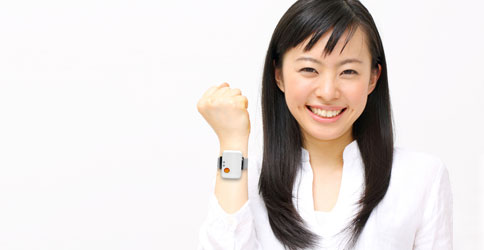
\includegraphics{images/shimmerphoto.jpg}
\caption{Product photo of the SHIMMER sensing platform.}
\label{Fig:ShimmerHand}
\end{center}
\end{figure}
Our application of using wrist movement to detect bites is very similar to biomedical research where the body is being monitored.
Similar constraints on the size of devices and battery life exist when they have to be used in biomedical research.
Burns et al. have demonstrated a device called the SHIMMER
(an acronym for Sensing Health with Intelligence, Modularity, Mobility and Experiment Resusability)~\cite{burns2010shimmer}.
The device is available in a small form factor (50mm X 25mm X 12.5mm),
and has a battery life of over twenty four hours with data from an accelerometer actively being recorded.
It features an MSP430 Ultra-low power microcontroller,
SD Card for storage,
a Bluetooth module for wireless communication,
and a lightweight battery (15).
It is possible to connect an external sensor to the SHIMMER by using its general purpose I/O pins.
Figure \ref{Fig:ShimmerHand} shows a product photograph of the device from the Shimmer website~\cite{Web:ShimmerBuyKit}.
Power is extended by disabling most components when not needed.
Burns et al. mention that the duty cycle of writing to the memory chip or the Bluetooth module can be reduced to save power,
however this is not possible in situations where the frequency is high because of the wake up time on these modules~\cite{burns2010shimmer}.
Shimmer sensing commercially provides these modules,
and a single base module can be purchased for US \$249~\cite{Web:ShimmerBuy}.
However, to program the SHIMMER base we would need access to the SHIMMER development KIT,
which costs US \$1999, or higher if additional features are required.



Since the device is to be worn by the user everyday, it needs to be comfortable to wear.
This would required the device to have a small size.
To avoid having to recharge often, or risking the battery dying during a meal,
the device also needs to have a good battery life\footnote{Requiring a recharge not more than once a day}.
Our device records raw inertial movement data (rotation and acceleration), and stores this in a memory chip.
The configuration of the various axes is displayed in Figure \ref{fig:HandAxis}.
The data can later be accessed later using a computer and can processed by algorithms
to detect when a bite of food has been eaten~\cite{dong2012new}.